\chapter[Literature Review]{Literature Review}
\label{Chap:2}
This literature review is broken up into three parts (I, II, and III), each one providing relevant information pertaining to the aims of the respective investigation incorporated as Chapters \ref{Chap:2}, \ref{Chap:3}, and \ref{Chap:4}. The aim of the investigation incorporated as Chapter \ref{Chap:2} was to compare the distribution of joint powers, muscle activity, and effective mechanical advantage between seated and non-seated postures during high power output cycling. Thus, Part I of the literature review will focus on the geometry and drivetrain of the bicycle, typical patterns of muscle activity and limb mechanics during cycling, and what is currently known about the non-seated posture. The aim of the investigation incorporated as Chapter \ref{Chap:3} was to understand the implications of mechanical energy changes of the rider's CoM on crank power output and limb mechanics during non-seated cycling at different power outputs and cadences. Thus, Part II will focus on why mechanical energy changes of the CoM may influence the total power output a rider must generate during cycling, and the unique influence that changing power output and cadence have on torque requirements during cycling. The aim of the investigation incorporated as Chapter \ref{Chap:4} was to understand how different constraints on lateral bicycle dynamics effect CoM movement and limb mechanics during non-seated cycling. Thus, Part III will focus on lateral bicycle dynamics, the effect of bicycle lean on the balance and stability of the bicycle, and the difference between riding outdoors, on a treadmill, and on rollers.

%%%%%%%%%%%%%%%%%%%%%%%%%%%%%%%%%%%%
\section{Part I}
%%%%%%%%%%%%%%%%%%%%%%%%%%%%%%%%%%%%

\subsection{Transmission and gearing}
    A machine achieves ideal mechanical efficiency when there is no loss of power during transmission \autocite{SimonMata2016}. A bicycle is an intricate example of excellent mechanical efficiency. The teeth of the front chain ring and rear sprocket, linked by a chain, send power produced by the rider to the rear wheel. A well-maintained bicycle will only lose approximately 2.3$\%$ of power during transmission \autocite{Martin1998}. These small power losses are due to the combination of friction, deformation, and wear within the frame and components.
    
    The mechanical advantage (MA) of the system dictates whether this power will then produce force or displacement at the rear wheel. The definition of MA is the ratio between the output force and the input force \autocite{SimonMata2016}. Four components of the bicycle contribute to its MA. They are the rear wheel (including the tyre), rear sprocket, front chain ring, and crank arm. A change in the radii of any of these components will cause a change in MA. Because the crank arm rotates in a circular path around its spindle, a change in its length is equal to a change in radius. These four components act around two axes of rotation, each with two gears. We can use the radii of these four components to calculate a bicycles MA as shown in Equation \ref{eq:MA} \autocite{SharpArchibald1977}.
    
    \begin{equation}
        \text{MA} = \frac{\text{Crank arm length (mm)} \cdot \text{Sprocket size (teeth)}}{\text{Rear wheel radius (mm)} \cdot \text{Chain ring size (teeth)}}
        \label{eq:MA}
    \end{equation}
    
    You can conceptualise MA as the ease at which you can pedal. If you ride a bike with a high MA on a flat surface it will feel very easy to pedal. The lower the MA the harder it is to pedal. Travelling at a certain velocity using an ``easy'' gear requires a higher cadence (measured in pedal revolutions per minute (rpm)) than using a ``hard'' gear. This is because the MA value dictates how much pedal displacement will occur per unit of rear wheel displacement. The inverse of MA is the gear ratio. In Equation \ref{eq:MA} we can see that an increase in crank arm length and/or rear sprocket size will increase MA as will a decrease in rear wheel radius and/or front chain ring size, thus, increasing the distance that the pedal must travel per unit of rear wheel displacement. In this scenario the rider trades displacement of the system for maximising force output. An example of this occurs when a rider cycles up a steep hill. The rider shifts the chain onto a smaller front chain ring or a larger rear sprocket to decrease the force required at the pedal. For instance, modern road bicycles commonly have a total of 22 gears, made up of two front chain rings and 11 rear sprockets. The MA of these modern road bicycles will range from 0.1 to 0.5. Riders can choose to alter the range and spacing of gears to suit the cycling event and their strengths. 
    
    The other important aspect of a bicycle's MA is the ratio of angular velocity between the wheels and the crank. Low MA allows the rear wheel to reach angular velocities that are unattainable by the rider at the pedal \autocite{SharpArchibald1977}. This is most helpful during flat sections, downhill descents, and fast sprint finishes. Altering the MA of the transmission allows a rider to achieve their desired power output using any combination of torque and angular velocity that the gearing and terrain allows. A later section on human power generation will discuss why riders choose certain combinations of torque and cadence.

\subsection{Phases of the crank cycle}
    ``Crank cycle'' is one term used to describe when the pedal completes a 360\textdegree revolution of the crank axis \autocite{Fonda2012}. Top dead centre (TDC, 0\textdegree) refers to the point in which the pedal is at its highest point during the crank cycle if the bicycle is on a level surface. TDC defines the start and end point of the crank cycle (0-360\textdegree). If the bicycle is on a level surface, then TDC will coincide with a vertical crank position, however, when on a slope the change in angular position of TDC will be equal to the slope of the riding surface. Bottom dead centre (BDC, 180\textdegree) is a term used to define the halfway point of the crank cycle. BDC also defines the end of the first phase, known as the downstroke (0-180\textdegree) and the start of the second phase, known as the upstroke (180-360\textdegree). These reference points allow spatial and temporal comparisons of biomechanical parameters during cycling.

\subsection{Geometry of the bicycle}
    The geometry and configuration of the bicycle dictate rider position during seated cycling \autocite{Muller2008}. Depending on the goals of the rider, the configuration will aim to maximise performance, comfort, or a blend of each \autocite{Too2003}. We can adjust five parts of the bicycle to position the legs: saddle height, saddle setback, crank length, spindle width, and cleat position \autocite{Hayot2012}. The position of the upper body will then rely on the position of the handlebars in relation to the saddle. 
    
    The effects of saddle height \autocite{Bini2014}, saddle setback \autocite{Rankin2010}, crank length \autocite{Barratt2016}, and cleat position \autocite{Straw2016} have all been thoroughly investigated. Yet, it has been difficult to isolate the effects of each variable due to the complex interaction between one another \autocite{Rankin2010}. For example, a change in crank length will also alter the angle and distance between the saddle and pedal during the crank cycle. Thus, it is understandable that research into these variables has yielded mixed results. 
    
    The influence of saddle height on lower limb kinematics during cycling is more consistent \autocite{Bini2011}. Research shows that saddle height has a significant effect on knee and ankle kinematics \autocite{Nordeen-Snyder1977}. A 5$\%$ decrease in saddle height can decrease extension of the knee by 35$\%$ \autocite{Nordeen-Snyder1977}. This will impact the length, rate of length change, and moment arm of knee extensor muscles \autocite{Bini2011}. Thus, pelvis to pedal distance may play an important role in joint mechanics and energetics during cycling \autocite{Hull1990}.
    
    An important consideration is that altering any of these variables may cause a change in both the horizontal and vertical position of the rider's CoM relative to the pedal. It may be that changing the position of the CoM relative to the pedal is a confounding variable that underlies any differences in metabolic energy expenditure or performance caused by changing these variables.  

\subsection{Muscle activity}
    Due to the constraint of the pedal trajectory during cycling, the basic phasing of functional muscle groups in the lower limb remains similar across different task demands \autocite{Raasch1999}. Riders will tend to concentrate their muscular effort during the downstroke to match the optimal force and power producing capabilities of the lower limb \autocite{Ericson1988,Yamaguchi1990}. Hip extensors, knee extensors, and ankle plantar flexors produce the majority of work to move the pedal from TDC to BDC \autocite{Ericson1988}. During the latter stages of the downstroke, knee flexors activate even though the knee continues to extend \autocite{Hug2009}. This hamstring activity during concurrent knee extension is known as Lombard's Paradox \autocite{Gregor1985}. Activating a knee flexor during knee extension would seem to be inefficient, however, the activation of bi-articular hamstring muscles (i.e. biceps femoris) is able to contribute to power output during the second half of the downstroke by redirecting the external force produced on the pedal \autocite{Gregor1985}. Thus, the coordinated activity of uni- and bi-articular muscles partially avoids the inefficiency of uni-articular muscles having to actively lengthen and absorb power during the downstroke, thereby increasing the efficiency of steady-state cycling \autocite{Kuo2001}. 
    
    It is also clear that the nervous system quickly adapts this paradoxical activity in response to changing task demands \autocite{Connick2013}. For example, it has been shown that the specific timing of bi-articular hamstring activity is sensitive to changes in both saddle height and cadence \autocite{Connick2013}. Knee extensors activate close to TDC in preparation for the downstroke. The activation of knee extensors continues through the downstroke to around 120\textdegree. This creates a large and effective knee extensor moment to drive the pedal. Hip extensors also activate around TDC and then peak at about 60\textdegree. This coincides with the pedal moving downward away from the hip joint. This hip extension moment continues through the downstroke to BDC. The ankle plantar flexors activate for a shorter period compared to hip and knee extensors; beginning after TDC, peaking at approximately 90\textdegree and ending after BDC. The transition to the upstroke then begins. Far less muscle activity occurs during the upstroke compared to the downstroke. Typically, the hip flexors, knee flexors, and ankle dorsiflexors produce relatively small amounts of work to return the pedal from BDC to TDC. The amount of effective tangential force applied to the pedal during the upstroke is minimal compared to the levels of flexor muscle activity \autocite{Hug2009}. This is because the pedal is raised predominantly by the action of the contralateral leg, which drives the opposite pedal downward from TDC to BDC. Thus, the hip flexors and knee flexors act predominantly to lift the leg during the upstroke to minimise counter-productive tangential pedal force.  
    
    Figure \ref{fig:emg} shows the electromyographical (EMG) activity measured in six lower limb muscles while cycling under three conditions: 1) seated on a level treadmill (LS), 2) seated on an inclined treadmill (US), and 3) non-seated on an inclined treadmill (ST) \autocite{Li1998}. It appears that changing incline has little effect on the pattern of lower-limb muscle activity, while there are large effects due to the change in posture; especially within the primary hip extensor, gluteus maximus, and the primary knee extensor, vastus lateralis.

    \begin{figure}[htbp]
    \centering
      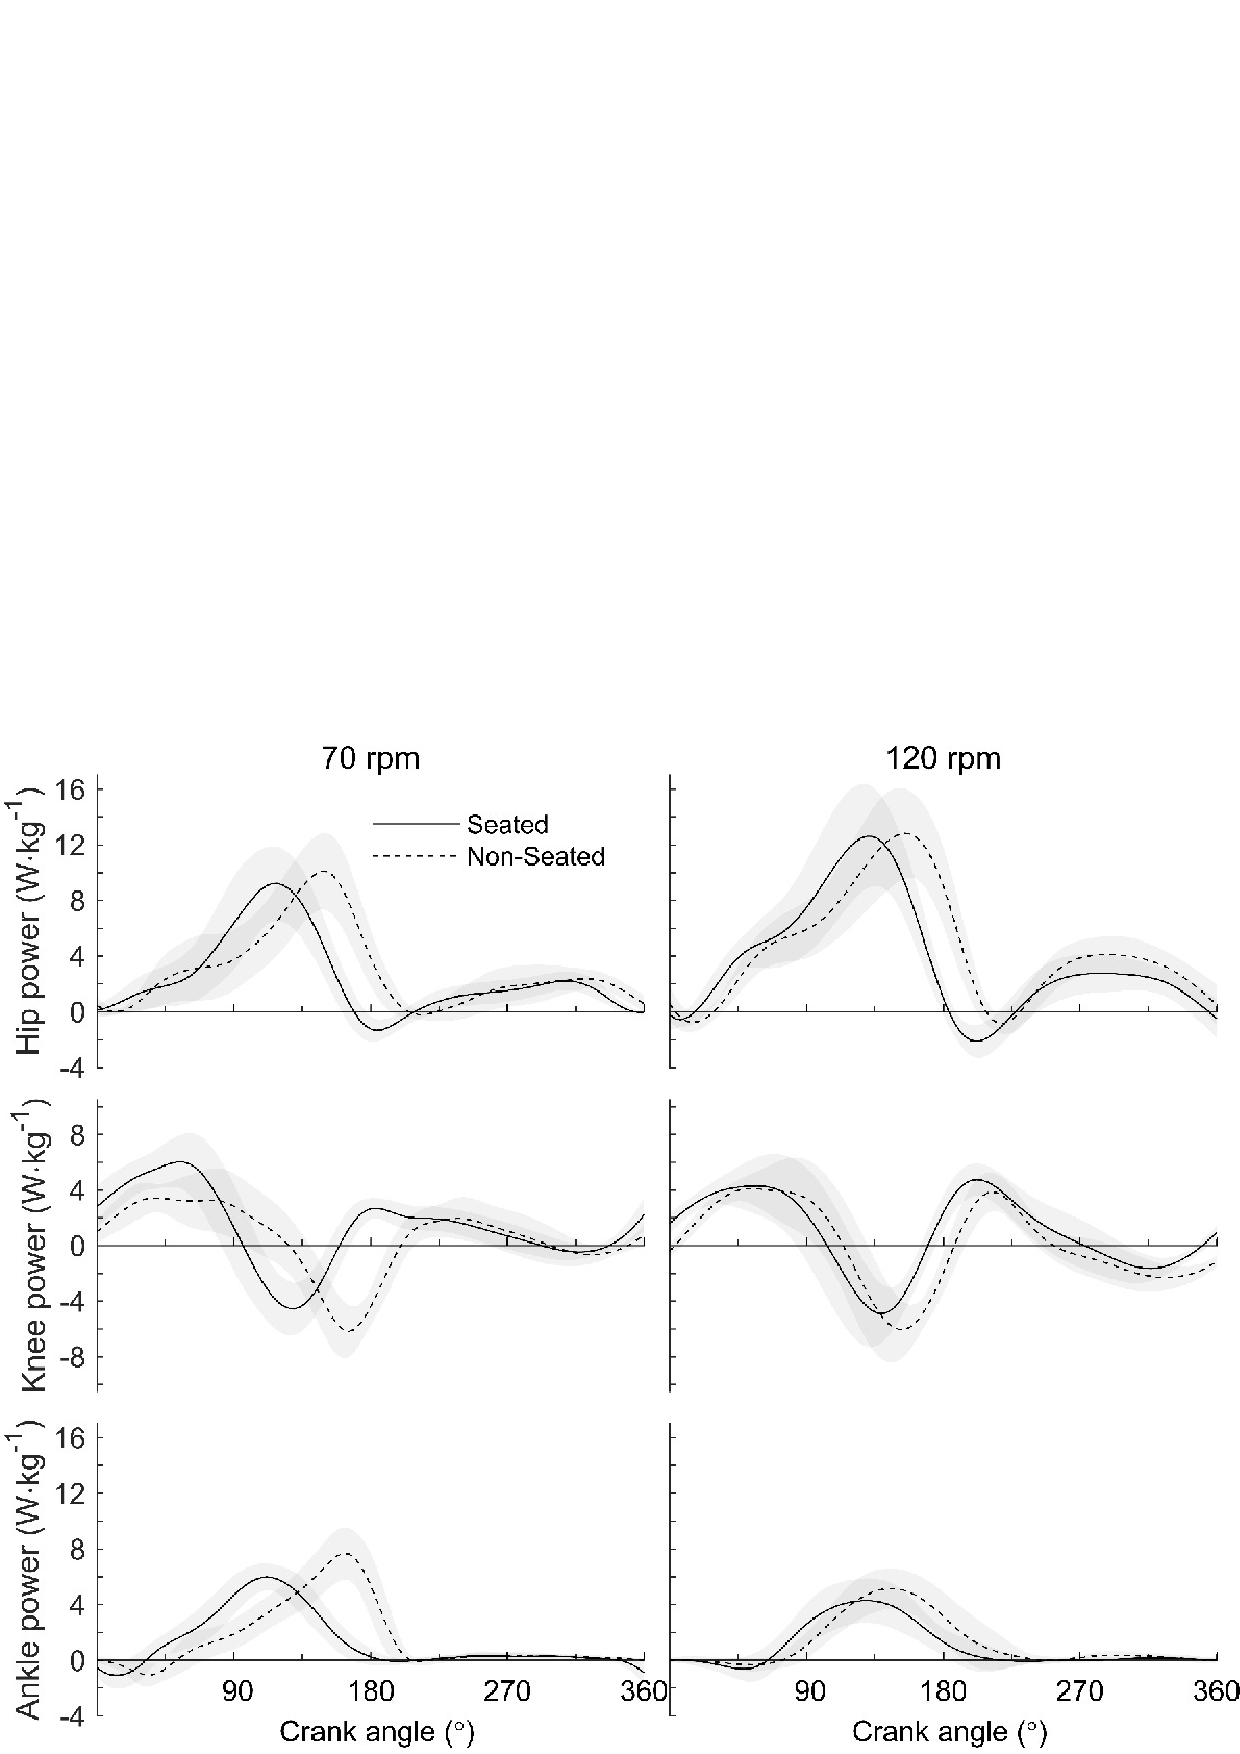
\includegraphics[width=0.4\textwidth]{LitReview/Figure2.png}
      \caption[Bi-articular muscle activation is extremely sensitive to changes in task demands.]{\textbf{Bi-articular muscle activation is extremely sensitive to changes in task demands.} Shown here is muscle activity within the lower limb during seated cycling on a level treadmill (LS), seated on an inclined treadmill (US), and non-seated on an inclined treadmill (ST). Note the altered pattern of rectus femoris activity due to the change in posture. \textit{Adapted [reprinted] with permission from Li L, Caldwell GE. Muscle coordination in cycling: effect of surface incline and posture. J Appl Physiol. 1998;85(3):927-34. Copyright \textcopyright 1998 by American Physiological Association.}}
      \label{fig:emg}
    \end{figure}
    \FloatBarrier

\subsection{Limb mechanics}
    \subsubsection{Muscle mechanics}
        During cycling, the rider assumes the role of an engine for the bicycle. The only mechanical structure in humans that can generate net positive mechanical power is muscle. Thus, we must consider the properties which govern a muscle's ability to generate power. Peak power and efficiency of a muscle are an extension of its force producing capabilities in relation to length and the rate of length change (velocity) \autocite{Hill1922}.
        
        If a muscle is fully activated, then the force a muscle exerts is primarily dependent on its size (physiological cross-sectional area (PCSA)), fascicle length, and the speed at which it contracts. During cycling, it is important to consider the collective force-length curve of a group of synergistic muscles rather than each muscle in isolation. The muscle group that contributes the most power during steady-state cycling is the knee extensor group \autocite{Ericson1988, Elmer2011}. The knee extensor group contains the bi-articular rectus femoris muscle, which means that the knee extensor strength curve is dependent on hip angle. The dependence of the knee extensor strength curve on hip angle will be proportional to the contribution of rectus femoris, which has a PCSA 92$\%$ the size of vastus lateralis and is larger than vastus medialis (128$\%$) and vastus intermedius (144$\%$) \autocite{Herzog1991}. A comparison of theoretical and experimental knee extensor strength curves by Herzog et al. (1991) showed that at a hip angle of 180\textdegree (lying with a straight leg) rectus femoris will produce maximal force at a knee angle of approximately 155\textdegree. With the hip fully extended, the rectus femoris will be the major contributor of knee extensor force at knee joint angles ranging from about 135\textdegree to full knee extension. At a hip angle of 90\textdegree (sitting) rectus femoris will produce maximal force at a knee angle of approximately 60\textdegree (full knee extension = 180\textdegree), and a complete loss of active force production due to the loss of overlap of the myofilaments within the sarcomeres will likely occur at a knee angle of approximately 135\textdegree. Furthermore, the rectus femoris will likely become the major contributor to knee extensor force at knee joint angles ranging from 80\textdegree to full knee flexion \autocite{Herzog1991}. Hence, it is important for cyclists to consider both their hip joint angle and knee joint angle when adjusting their riding posture and bicycle geometry in order to ``optimize'' the strength curve of the knee extensor group.
        
        Muscles convert chemical energy to mechanical energy at an efficiency of around 20-25$\%$ \autocite{Wilkie1950}, but this efficiency can drop to zero if an external force is so large that the muscle cannot move it. Thus, to utilise the greatest efficiency of muscle, we must match the force and velocity of movement to produce the most power. Peak efficiency occurs at approximately 50$\%$ of peak force and approximately 25$\%$ of peak shortening velocity \autocite{WILKIE1960b}, but peak power production will occur at higher shortening velocities than that of peak efficiency \autocite{WILKIE1960b}. 
    
        Human potential for mechanical power output decays exponentially as a function of activity duration \autocite{WILKIE1960a, Harrison1970}, which affects the the optimal force and velocity of movement \autocite{Too2003}. For instance, maximal power output occurs at a cadence of approximately 120 rpm \autocite{McCartney1983,Gardner2007}. As power output decrease over time, so too does the cadence that maximises power output \autocite{MacIntosh2000}. At sub-maximal power outputs, elite cyclists tend to cycle at a higher cadence than that which is most metabolically efficient \autocite{Marsh1993}. Yet, these higher cadences lead to a greater time to exhaustion \autocite{Nickleberry1996}. Surprisingly, it is only when cycling uphill that riders tend to reduce their preferred cadence closer to that which is most efficient \autocite{Lucia2001}. Research suggests that preferred cadence may be related to a number of factors including joint-moment minimisation, muscle power, and gross efficiency \autocite{Marsh2000a}, but it remains unclear which factor is being prioritised by the rider and whether this changes under different task constraints.

    \subsubsection{Segmental energy transfer}
        During cycling, muscles create pedal force through the proximal-to-distal transfer of segmental energy \autocite{Enoka2008,Kautz2002}. Thus, the leg muscles are required to produce, absorb, and redistribute energy. The type of contraction that the muscle undergoes will dictate the ratio of energy distributed from one connected segment to another. A concentric (shortening) contraction produces mechanical work. This means that an accelerated segment will gain more energy than that lost by the connected decelerated segment. The opposite will occur for an eccentric (lengthening) contraction, which will absorb energy. An isometric (fixed length) contraction will redistribute an equal amount of energy between segments \autocite{Zajac2002}. 
        
        The synergy of muscle activity in the lower limb can increase the amount of force produced on the pedal. For example, the synergistic activity of the triceps surae redistributes work done by the gluteals and vastii on the thigh and shank, respectively, to the pedal. This enables the transfer of energy across the ankle to the pedal. Without this activity the angular momentum of the thigh and shank would force the ankle into dorsiflexion \autocite{Zajac2002}. Bi-articular muscles and the co-activation of muscles on opposing sides of the joint complicate the transfer of energy between segments. This makes it difficult to categorise muscles as having distinct functional roles during cycling. Nevertheless, comparing the magnitude and patterns of muscle activity under different cycling conditions can reveal important insights into the pattern of segmental energy transfer and the role of particular muscles during cycling.  
        
        \begin{figure}[htbp]
        \centering
          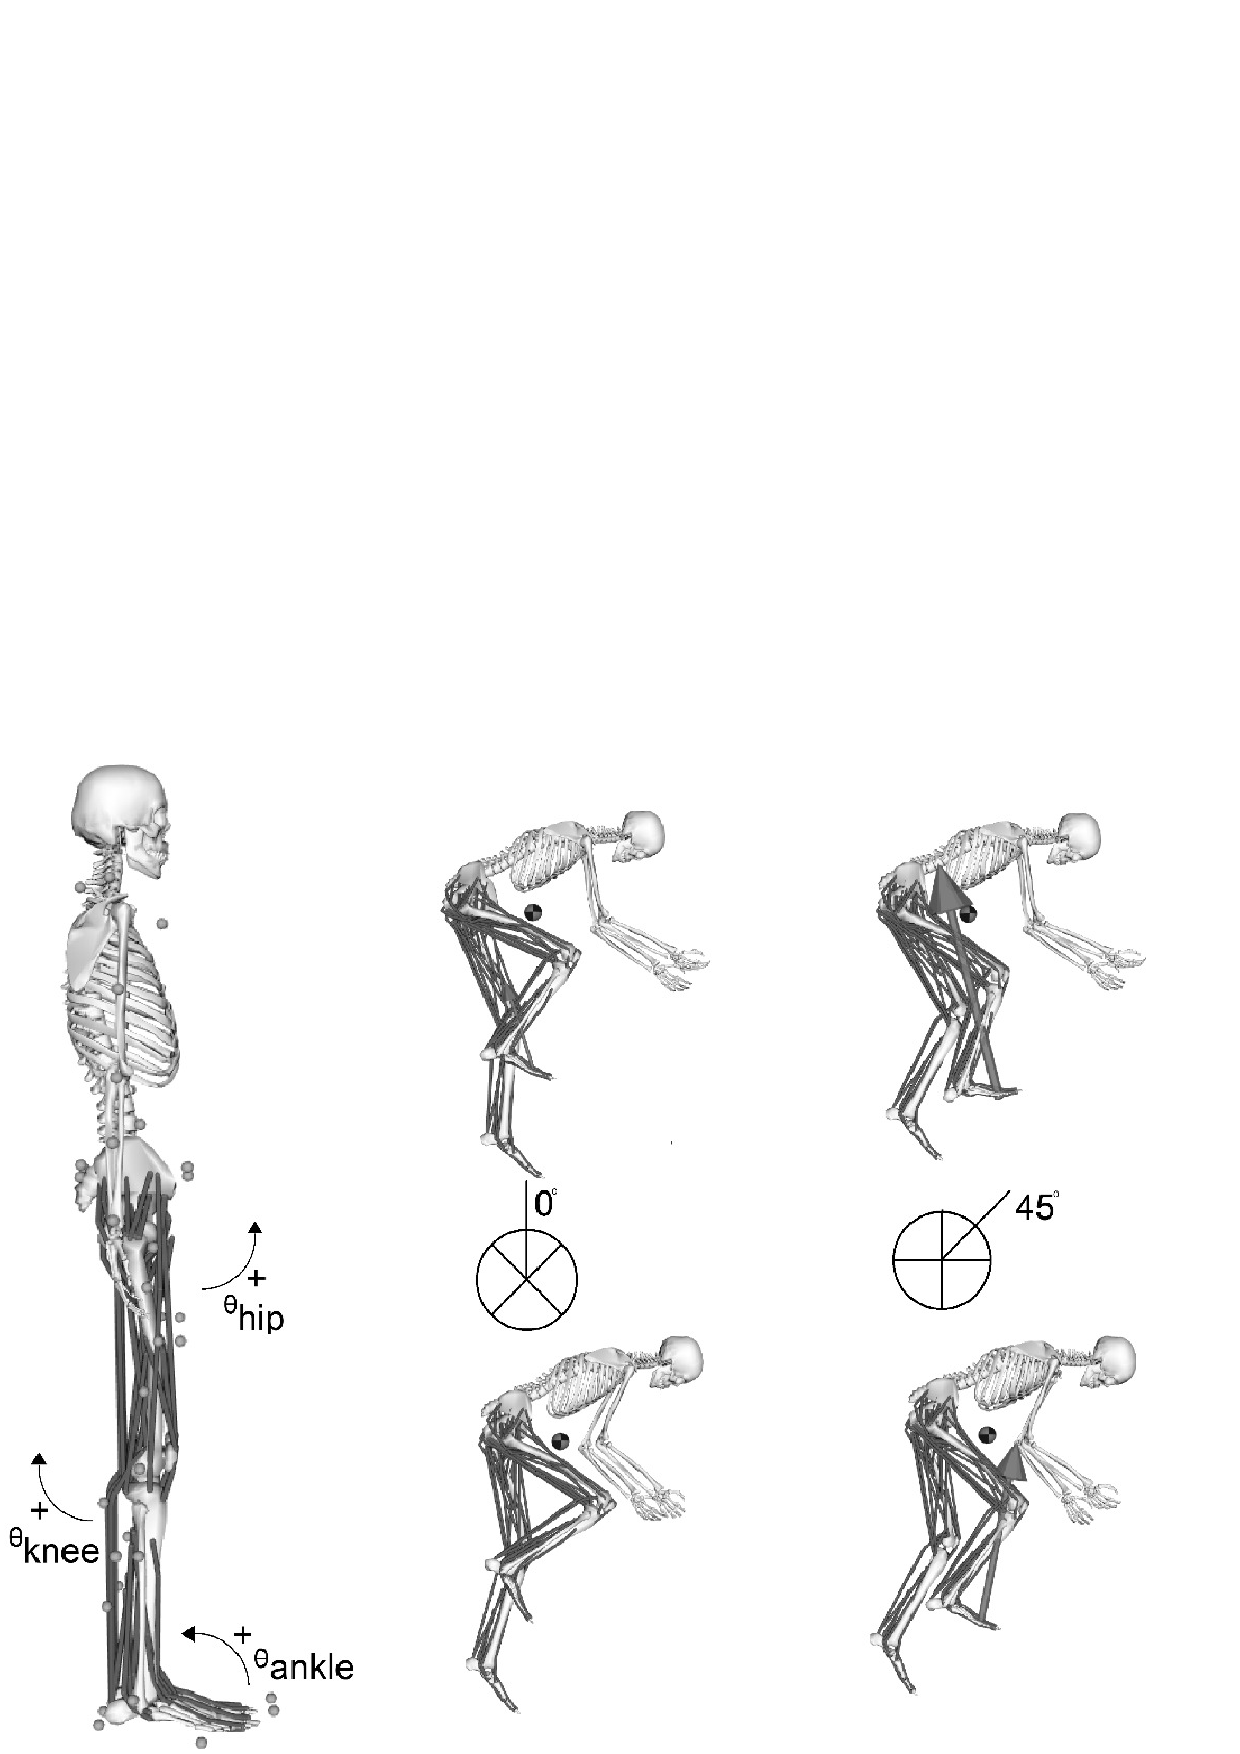
\includegraphics[width=0.8\textwidth]{LitReview/Figure1.png}
          \caption[Bi-articular muscles act to control the direction of external force at the pedal.]{\textbf{Bi-articular muscles act to control the direction of external force at the pedal.} Depiction of how bi-articular muscles act to control the direction of the external force vector. Rectus femoris can act to transfer hip extension power to the knee, while biceps femoris long head can transfer knee extension power to the hip. F$_G$, Pedal reaction force. \textit{Adapted [reprinted] with permission from Van Ingen Schenau GJ, Boots PJM, de Groot G, Snackers RJ, and van Woensel WW. The constrained control of force and position in multi-joint movements. Neuroscience. 1992;46(1):197-207. Copyright \textcopyright 1992 by Elsevier.}}
          \label{fig:biarticular}
        \end{figure}
        \FloatBarrier

    \subsubsection{Directing external force output}
        Cycling is an interesting example of an ``open-chain kinetic exercise'' \autocite{Enoka2019} whereby pedalling efficiency relies on both the magnitude and direction of pedal force. Thus, coordinating the intensity and timing of muscle activity in the lower limb is crucial to the task. The resultant pedal force is made up of both tangential and radial force; the direction of which are perpendicular and parallel to the crank, respectively. The circular trajectory of the pedal means that only tangential force is effective in producing forward motion \autocite{Gregor2011}. The primary force producing muscles of the lower limb alone cannot produce an effective force throughout the pedal cycle \autocite{Zajac2002}. Thus, there is a need for co-contraction of uni- and bi-articular muscles to control the size and direction of the pedal force vector \autocite{VanIngenSchenau1990a}. For example, the production of an effective force at the start of the downstroke requires a large net knee extensor moment. During the second half of the downstroke, hip extensor, knee flexor, ankle plantar flexor moments act to direct the pedal force vector perpendicular to the crank. 
        
        Muscle activity can also lead to the production of radial force. Although radial force is not effective at turning the crank, the theory that reducing the ratio of radial to tangential force (often referred to as ``force effectiveness'') will increase efficiency and performance is fundamentally flawed \autocite{Kautz1993}. The main oversight in this theory is that radial force is often generated by non-muscular forces such as momentum of the lower limbs \autocite{Neptune2000}. This means that any attempts to offset this non-muscular force would require greater muscular effort to decelerate the lower limb segments \autocite{Kautz1993}. It is likely that attempting to control the momentum of the segments in this manner would place a greater demand on muscle and decrease a rider's time to task failure at a given mechanical power output \autocite{Enoka2019}.
    
    \subsubsection{Effective mechanical advantage}
        Postural changes can affect the required muscle force during many forms of terrestrial locomotion \autocite{Alexander1991,Kram1998,Kipp2018}, which subsequently affects metabolic cost \autocite{Biewener2004}. These postural changes can affect the amount of muscular force needed by altering the MA of the lower limb \autocite{Biewener1989}. The MA of a muscle is calculated as the ratio of the reaction force moment arm to the muscle moment arm, known as ``effective mechanical advantage'' (EMA) \autocite{Biewener1989}. The muscle moment arm is the perpendicular distance from the muscle-tendon insertion to the joint centre. The reaction force moment arm is the perpendicular distance from the projection of the ground reaction force to the joint centre. 
        
        Research has shown that runners are able to minimize their energetic cost by increasing the overall EMA of the lower limb \autocite{McMahon1987}. They achieve this through a reduction in the ground reaction force moment arm. During stance phase, runners align the ground reaction force vector with the longitudinal axis of the support leg \autocite{Chang2000}. A key difference between running and cycling is that a saddle supports the majority of a cyclist's bodyweight. This will reduce the effect of bodyweight on the magnitude and direction of the pedal reaction force. This means that transition from a seated to a the more vertically aligned non-seated posture is likely to increase EMA of the lower limb during cycling. To the best of our knowledge, no data currently exists on EMA during cycling in either a seated or non-seated posture.
    
    \subsubsection{Joint-specific power}
        The biomechanics of cycling are typically studied under power outputs associated with steady-state exercise or maximal endurance performance \autocite{Bini2014}. Yet, cycling events are usually interspersed with brief but important periods of high power output, such as accelerations, climbing, and sprinting \autocite{Lucia2003}. Thus, many gaps still remain pertaining to the biomechanics of cycling at high power outputs. Knee extensors contribute the most power during the pedal cycle at low to moderate power outputs \autocite{Ericson1986}. However, hip extensors become the largest contributor at high power outputs \autocite{Martin2009, Elmer2011}. This redistribution of joint power may occur due to an increase in knee flexor moments, which reduce the knee extensor moment and subsequent net knee power, or the ability of hip extensors to produce higher maximal joint moments than the knee extensors \autocite{Anderson2007}. Figure \ref{fig:jointpower} shows the patterns of joint-specific power in response to increasing power output at a cadence of 90 rpm. As expected, all joint powers increase with an increase in power output, but the relative increase in peak hip power is much larger than at the knee or ankle. These results may provide a clue as to why cyclists spontaneously transition from a seated to a non-seated posture at high power outputs. If joint power is redistributed away from the knee when cycling in a seated posture as power output increases, then it is possible that this re-distribution of joint power could be linked to the transition response of riders. To date, joint-specific power during non-seated cycling has not been published. Further consideration should also be given to the effects of changing cadence on joint-specific power during seated and non-seated cycling.  
        
        \begin{figure}[htbp]
          \begin{center}
          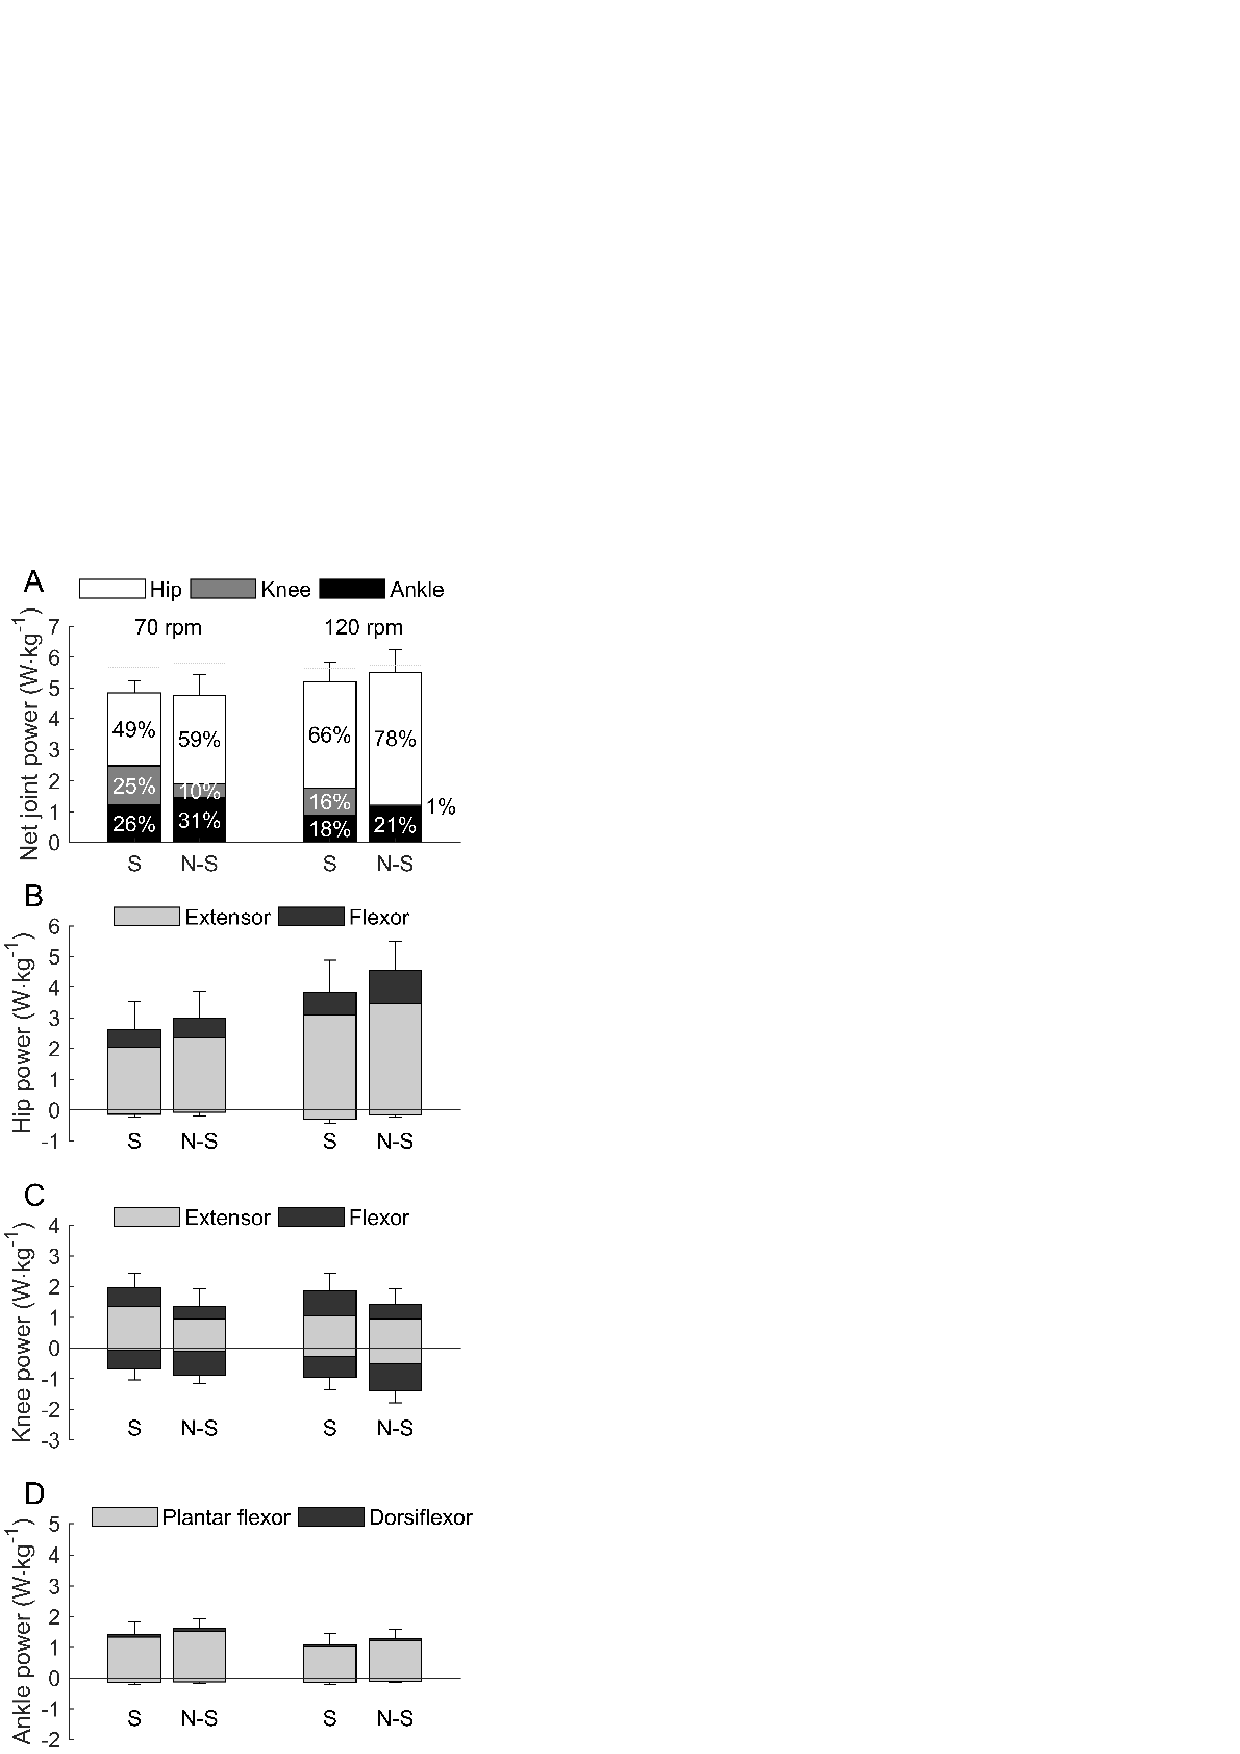
\includegraphics[width=0.48\textwidth]{LitReview/Figure3.png}
          \end{center}
          \caption[During seated cycling, joint power is redistributed away from the knee to the hip as power output increases.]{\textbf{During seated cycling, joint power is redistributed away from the knee to the hip as power output increases.} Shown here are the patterns of joint-specific power within the lower limb during seated cycling at 90 rpm as power output is increased from to 250 Watts, through 850 Watts, to Maximum. \textit{Adapted [reprinted] with permission from Elmer SJ, Barratt PR, Korff T, and Martin JC. Joint-specific power production during sub-maximal and maximal cycling. MSSE. 2011;43:1940-1947. Copyright \textcopyright 2011 by Wolters Kluwer Health, Inc.}}
          \label{fig:jointpower}
        \end{figure}
        
        The time that the lower limb and each joint spends in extension was also shown to increase at high power outputs \autocite{Elmer2011}. This increases the time spent using stronger anti-gravity muscles to generate power \autocite{Yamaguchi1990}. The ratio of time a joint spends extending relative to flexing is known as the duty cycle. Thus, it is proposed that an increase in duty cycle is an essential strategy for producing maximal power. To date, duty cycle values during non-seated cycling have not been published.
        \FloatBarrier
    
\subsection{Non-seated posture}
    During short, intensive bouts of cycling, many riders choose to ride out of the saddle \autocite{Harnish2007}. Single-day or multi-stage road races can often end with enthralling high-speed or steep uphill sprints to the finish. In some cases, two riders will go head-to-head while in two different postures; one seated while the other is not. It is a fascinating scenario, which leads one to ask whether the choice of posture is a key factor in the result. This question has led many researchers to try and understand the effects of the non-seated posture on cycling performance \autocite{Tanaka1996,Li1998,Millet2002,McLester2004,Poirier2007,Hansen2008,Turpin2016}.
    
    It has been shown that recreational cyclists will transition to a non-seated posture at a power output of approximately 567 Watts at a cadence 90 rpm \autocite{Costes2015}. Yet, it has been proposed that cyclists should transition well before this power output to increase performance \autocite{Hansen2008}. One group of researchers compared time to exhaustion between the seated and non-seated posture at different power outputs \autocite{Hansen2008}. This study had elite cyclists ride to exhaustion on a treadmill set with a 10$\%$ gradient in either a seated or non-seated posture. Different intensities were set relative to the highest power output the subject could sustain for one minute (W$_{max}$). Most riders in this study achieved a greater time to exhaustion using a non-seated posture at their W$_{max}$ intensity or above. W$_{max}$ equated to a power output of 441 Watts for this subject group. Thus, it is possible that a non-seated posture may enhance performance fatigability \autocite{Enoka2019} within lower-limb muscles when cycling at power outputs above the preferred transition power. Based on their findings, the authors recommended that cyclists should use the non-seated posture when riding above 94$\%$ of W$_{max}$. However, previous research has found no difference in gross efficiency between a seated and non-seated posture at power outputs equivalent to only 75$\%$ of W$_{max}$ \autocite{Millet2002}.
    
    There is also a difference in the preferred cadence used during seated and non-seated cycling \autocite{Hansen2008}. At W$_{max}$ subjects dropped their cadence from 97 rpm when seated to 71 rpm in a non-seated posture. Other research supports this finding, showing that highly trained and elite cyclists prefer to use a lower cadence when in the non-seated posture \autocite{Harnish2007,Lucia2001}. More recent research observed a much higher transition point of 567 Watts when controlling cadence at 90 rpm \autocite{Costes2015}. The discrepancy between this result and that of previous research suggests that cadence likely affects the preferred transition power. It must be noted that many other constraints may explain the difference in these results including slope, riding experience, rider mass, ergometer type, activity duration, and fatigue. Further consideration should be given to the task constraints that may affect the preferred seated to non-seated transition power in cycling.
    
    \begin{figure}[htbp]
        \centering
        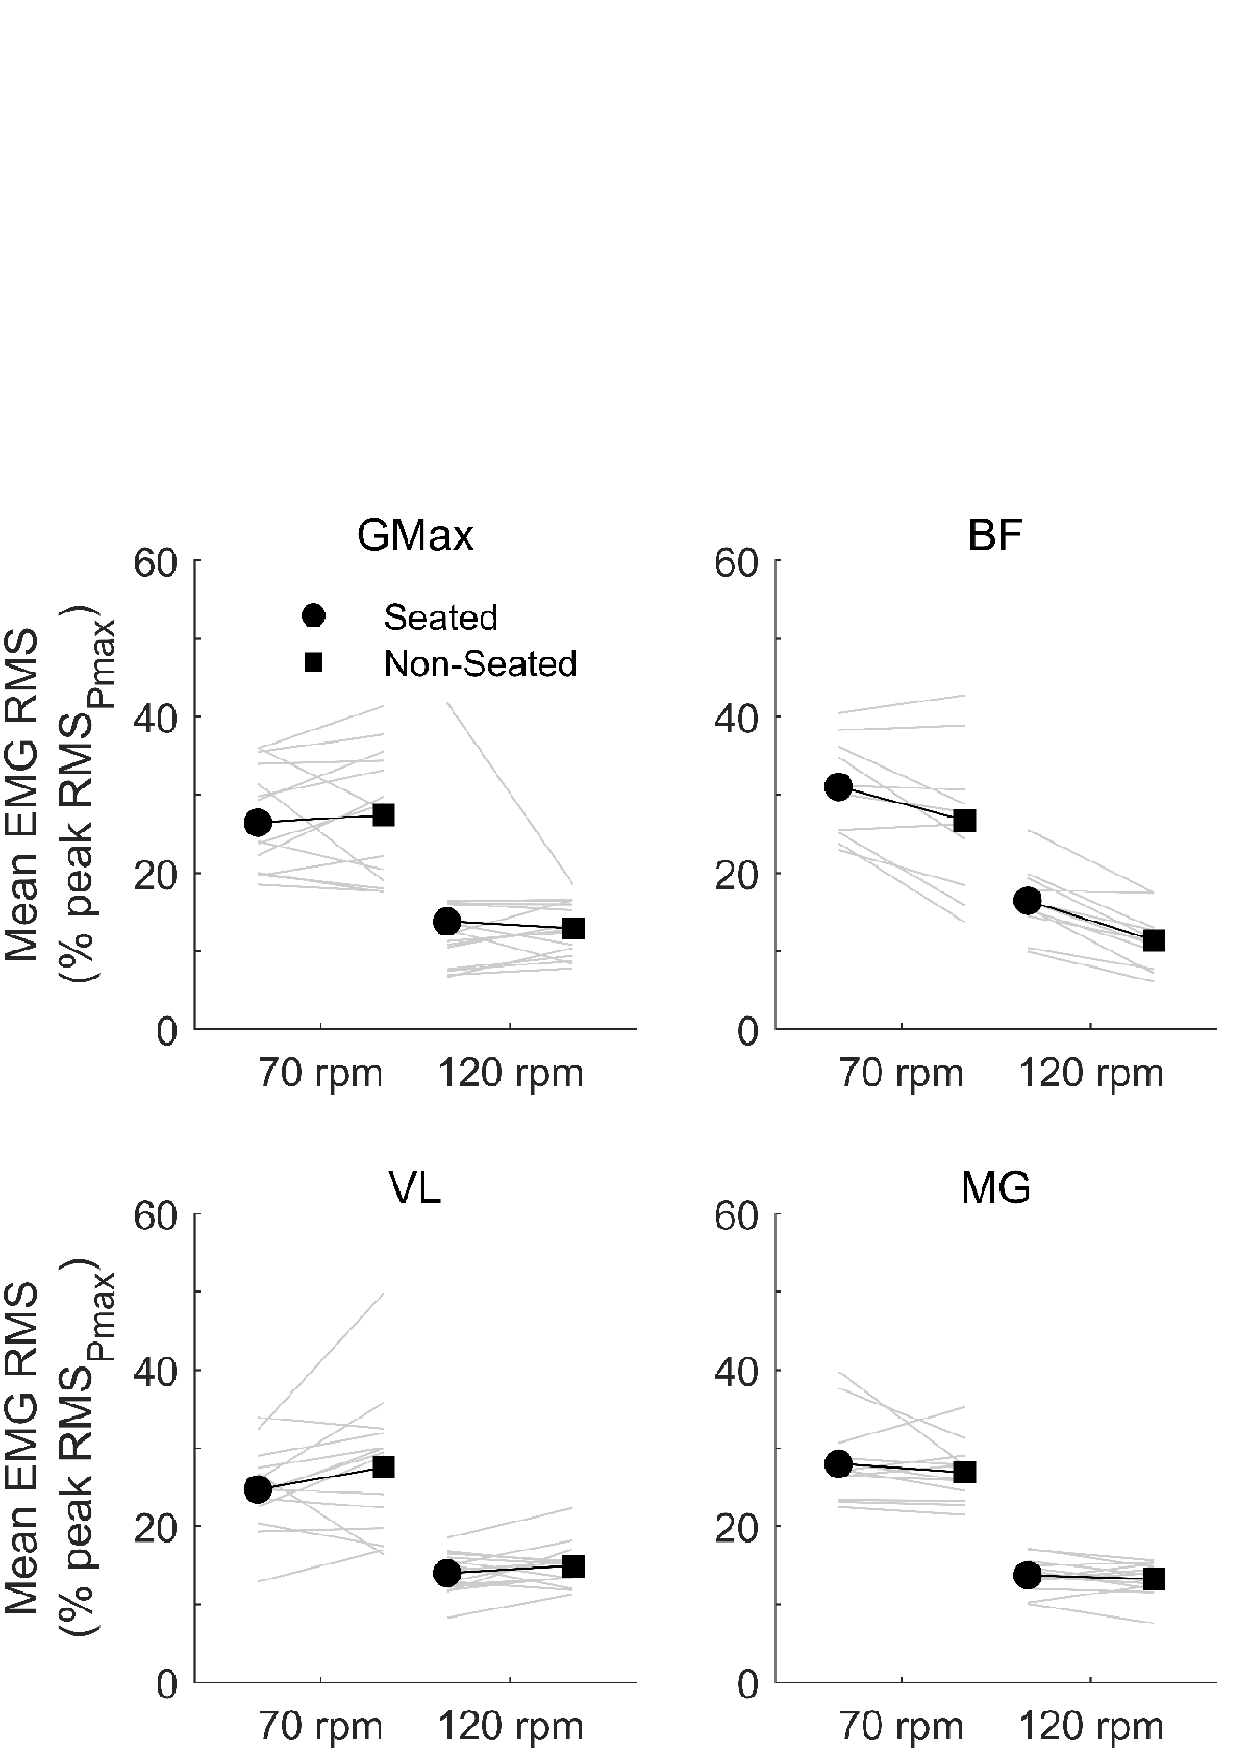
\includegraphics[width=0.6\textwidth]{LitReview/Figure5.png}
        \caption[Significant vertical displacement of a rider's CoM is likely to occur during non-seated cycling.]{\textbf{Significant vertical displacement of a rider's CoM is likely to occur during non-seated cycling.} Indirect evidence of vertical CoM displacement during non-seated cycling via the measurement of a pelvis marker. \textit{Adapted [reprinted] with permission from Hull ML, Beard A, Varma H. Goniometric measurement of hip motion in cycling while standing. J Biomech. 1990;23(7):687-703. Copyright \textcopyright 1990 by Elsevier.}}
        \label{fig:pelvis}
    \end{figure}
    
    Forward modelling of cycling has shown that the instantaneous power output at the pedal can exceed that of muscular power capabilities \autocite{Neptune1998}. This would suggest that lower-limb muscles are able to transfer energy of lower- and upper-body segments to the pedal. Pioneering research using cine film showed a sinusoidal pattern of vertical lower back displacement during over-ground non-seated cycling \autocite{Soden1978}. This finding was later confirmed by a study \autocite{Hull1990} on pelvis motion during non-seated cycling on a treadmill. Figure \ref{fig:pelvis} shows the results of pelvis midpoint elevation over one crank cycle. The vertical fluctuations of the pelvis indicate that substantial amounts of mechanical energy could also be gained and lost by the torso. Note the double cycle pattern of peak elevation and downward acceleration occurring during the downstroke. These results suggest that mechanical energy of the upper body may be transferred to the crank during non-seated cycling. More recent research using modern motion capture techniques have shown vertical motion of the trunk and hips increases with power output even when cycling in a seated posture \autocite{Costes2015}. Vertical displacement of the rider's CoM and the associated mechanical energy changes may affect the kinematics, kinetics, and energetics of the lower limb during both seated and non-seated cycling.
    
    A rider's CoM moves forward and upward when transitioning from a seated to a non-seated posture \autocite{Caldwell1999}. Evidence suggests that this leads to a phase shift of muscle activity and crank torque to later in the crank cycle \autocite{Li1998}. Fore-aft CoM displacement will change the ratio of bodyweight supported at the pedals versus the handlebar. The force vector due to gravity acting on the mass of the body is always directed towards the centre of the earth, which means any fore-aft movement of the CoM will change the moment arm between the CoM and the axis of crank rotation. Presumably, this change in moment arm could increase the contribution of a rider's body mass to pedal force, and subsequently increase time to exhaustion during high-power output cycling \autocite{McLester2004,Hansen2008}. It may also explain why cyclists report a lower perceived rate of exertion in the lower limb during non-seated cycling \autocite{Tanaka1996}. There is a need to test whether these measures relate to either an increase in peak maximal power or a decrease in peak total joint power generated by the rider during non-seated cycling.
    
    When in a non-seated posture, the bodyweight of the rider is supported by the pedals and handlebar. Partitioning out the separate metabolic costs of supporting bodyweight and accelerating body mass during running has provided important insights into running performance \autocite{Kipp2018}. However, quantifying the energy cost of producing force to support bodyweight seems to be far more complex when pedalling a bicycle than when on solid ground. Nevertheless, applying a similar approach to non-seated cycling may provide important insights into how muscle simultaneously supports bodyweight and generates net positive mechanical work to propel the bicycle during non-seated cycling. 
    
    Both efficiency and maximal power output are important aspects of cycling performance. Depending on the goal of the cycling task a rider may choose to prioritise one or the other. For instance, during very short sprints and climbs the priority may be to produce maximal power no matter the energetic cost. In this case, research shows that the non-seated posture is superior to the seated posture for producing maximal power \autocite{Millet2002}. It is also likely in this case, for chemical energy to be liberated primarily through anaerobic metabolism. Thus, comparisons of aerobic energy expenditure between the seated and non-seated posture are unlikely to reveal any advantage to the non-seated posture under steady-state conditions \autocite{Ryschon1991}. Rather, comparisons of lower-limb mechanics between the two postures may provide more insight into the preference for a non-seated posture.

%%%%%%%%%%%%%%%%%%%%%%%%%%%%%%%%%%%%%%%%%%%%%
\section{Part II}
%%%%%%%%%%%%%%%%%%%%%%%%%%%%%%%%%%%%%%%%%%%%%
\subsection{Human power output during cycling}
    Both internal and external forces impede forward motion of the bicycle. Positive power generated by muscle is dissipated to the environment (excluding gravity), to conservative forces (including gravity and the stretching of elastic elements), and to non-conservative forces such as friction and drag \autocite{VanIngenSchenau1990b}. To start moving forward, the rider must produce enough thrust to overcome resistance due to aerodynamic drag, rolling resistance, wheel-bearing friction, changes in potential energy, and changes in kinetic energy \autocite{Martin1998}. The portion of resistance attributed to these sources varies depending on the riding scenario. In most cases when riding on a flat surface, the main resistance will be due to aerodynamic drag. Atmospheric sources of drag include air density as well as the direction and velocity of wind. The total amount of drag experienced by the bicycle-rider system will depend on the velocity relative to wind, frontal surface area, and shape. The force needed to overcome aerodynamic drag increases to the square of velocity \autocite{Martin1998, Muller2008}. Thus, optimising shape and frontal surface area will decrease the power required per unit of velocity. For example, when travelling at a constant velocity of 30 km$\cdot$h$^{-1}$ (8 m$\cdot$s$^{-1}$) on a flat surface into a 2 m$\cdot$s$^{-1}$ head wind, approximately 75$\%$ of power production is needed to overcome aerodynamic drag \autocite{Martin1998}. At speeds above 50 km$\cdot$h$^{-1}$, drag increases to $>$90$\%$ of the total resistive force \autocite{Faria2005}. During steep uphill cycling the main resistance becomes the rate at which the rider gains potential energy due to gravity. When accelerating from a standstill on flat ground the main resistance is the rate of change in kinetic energy. Hence, a rider's choice of riding posture often depends on the type and magnitude of external resistance.
    
    Typically it is assumed that the rider's CoM travels parallel to the riding surface, meaning that the change in potential and kinetic energy of the rider's CoM is reflected by the change in the potential and kinetic energy of the system. Under this assumption power measured at the cranks will be equivalent to the total power output generated by the rider. However, this assumption does not account for any movement of the rider's CoM relative to the reference frame of the bicycle. Evidence suggests that this is particularly important when cycling in a non-seated posture as the rider's CoM is raised and lowered periodically during the crank cycle \autocite{Soden1978,Hull1990}. Thus, the total power generated by the rider (P$_{tot}$) will be equivalent to power measured at the cranks (P$_{cranks}$) plus the rate of energy gained and lost by their CoM (P$_{CoM}$) as shown in Equation \ref{eq:Ptot}
    
    \begin{align}
        P_{tot} = P_{cranks} + P_{CoM} \label{eq:Ptot} \\
        P_{lb} + P_{ub} = P_{cranks} + P_{CoM} \label{eq:Plb}
    \end{align}
    
    Typically, P$_{cranks}$ is calculated as the summed dot product of torque and angular velocity measured at each crank. P$_{CoM}$ is calculated using inverse kinematic results as the sum of the change in potential energy (E$_p$) and kinetic energy (E$_k$) of each segment divided by the change in time. P$_{tot}$ can also be thought of as the sum of lower body and upper body joint power as shown in Equation \ref{eq:Plb}. Lower body joint power (P$_{lb}$) can be calculated using inverse dynamic results as the summed dot product of net joint moments and joint angular velocities at the hip, knee, and ankle of each leg. Upper body power (P$_{ub}$) can be assumed to be the difference between P$_{tot}$ and P$_{lb}$, which can be attributed to the net power generated by muscles crossing the joints within the arms and trunk. It is far less common for studies to directly measure P$_{ub}$. The limitation of this is that it cannot be identified whether power is being simultaneously generated and dissipated within the upper body.
    
\subsection{Centre of mass movement during cycling}
    Contrary to popular belief, the CoM of the rider does not travel parallel to the riding surface even during seated cycling \autocite{Costes2015}. The measurement of rider kinematics during seated cycling shows that a rider's CoM is displaced in all three axes \autocite{Telli2016}. The vertical component of this displacement may have a significant energetic cost due to the energy required to raise the body's mass against gravity. As pedal torque increases the vertical displacement of the trunk also increases \autocite{Costes2015}. Limiting CoM displacement has been proposed as an optimal strategy during walking and running \autocite{Saunders1952}. Yet, adapting gait to constrain CoM movement can be even more costly than allowing CoM movement, as evidenced by ``Groucho'' running \autocite{McMahon1987}. If you can imagine walking with similar knee flexion angles used in seated cycling it may look like what has been termed ``Groucho'' running. This unusual gait was adopted by runners who were under instruction to run while limiting CoM movement. Subjects chose to run in a crouched posture with a compliant knee. This resulted in greater knee flexion angles than a preferred gait. This happened to be an excellent strategy for limiting CoM movement, however, this gait came at a higher energetic cost due to the increase in work required at the knee joint \autocite{Gordon2009}. These increased knee flexion angles led to an increase in knee extensor moments compared to a preferred gait. A similar concept could be tested during cycling, by instructing riders to limit CoM movement during non-seated cycling.
    
    Vertical acceleration of the rider's CoM during seated and non-seated cycling would mean that the full bodyweight of the rider is not always supported by the saddle and handlebars. There is evidence of this during seated cycling, where it was shown that, at a power output of 682 $\pm$ 111 W and a cadence of 90 rpm, the amount of bodyweight supported at the saddle was measured to be as low as 7 $\pm$ 5$\%$ \autocite{Costes2015}. Due to the flexed position of the leg during seated cycling, the loss of saddle support to this extent could significantly increase the force and work requirements of anti-gravity muscles. Presumably a more flexed hip and knee would decrease EMA, which would increase the muscle force required to support the greater portion of bodyweight at the pedals.
    
    Measuring a rider’s CoM position while cycling on an ergometer, treadmill, or over-ground can be done using an optical motion capture system. However, there are limitations to each of these experimental setups. Although ergometers allow multiple cycles to be collected per trial, they constrain the lateral dynamics of the bicycle, which changes the preferred movement pattern of the rider and may affect performance. Treadmills can provide a solution to ecological validity, but performing maximal sprinting is problematic due to the danger of matching the belt velocity to the rapid acceleration and high velocity of the bicycle wheels. Over-ground cycling can be captured, but the calibrated volume of the camera system will limit the number of cycles that can be collected. Thus, a method for tracking a rider’s CoM motion when motion capture is not feasible would make it possible to examine the preferred movement pattern of cyclists outside of the laboratory. A possible solution to this problem is presented in Appendix \ref{Chap:B}, where we undertook an additional study to assess the validity of an inertial measurement unit (IMU) mounted near the sacrum for measuring vertical CoM displacement and associated energy changes of cyclists while riding in a non-seated posture by comparing the derived vertical displacement of the IMU to an attached marker cluster tracked with an optical motion capture system and to a kinematic estimate of vertical CoM displacement using a full-body musculoskeletal model.
    
    Currently we can only speculate about the role of CoM movement during cycling. Research on this matter may shed light on whether the seated posture becomes unfavourable compared to a non-seated posture due to the bodyweight of the rider becoming unsupported at the saddle. Presumably as power output increases at a particular cadence, so too will the vertical component of pedal force. The upward accelerations of the CoM due to vertical pedal force may be detrimental for external power production if they occur during the downstroke, as this would require additional power to that generated on the crank. Transitioning to a non-seated posture could be an optimal strategy for generating high power outputs as the rider may be able to use their arms more effectively to resist upward accelerations of their CoM \autocite{Baker2002}.
        
\subsection{The effect of changing power output and cadence on crank torque}
    During cycling, the combination of power output and cadence dictates the amount of torque a rider must produce on the crank. Figure \ref{fig:torque} shows a surface plot of the crank torque required at a wide range of power output (50-1000 Watts) and cadence (20-160 rpm) combinations. Equation \ref{eq:Tcranks} shows how crank torque is calculated from power output and cadence.
    
    \begin{equation}
        T = \frac{P}{\omega} \label{eq:Tcranks} \\
    \end{equation}
    
    Where T is the mean torque over a crank cycle in Newton$\cdot$metres, P is the mean power output over a crank cycle in Watts,  and $\omega$ is the mean angular velocity over a crank cycle in rad$\cdot$s$^{-1}$. In Figure \ref{fig:torque} angular velocity ($\omega$) has been converted to cadence in revolutions per minute (rpm) using Equation \ref{eq:RPM}.
    
    \begin{equation}
        \text{Cadence (rpm)} = \frac{\omega \cdot 60}{2\pi} \label{eq:RPM} \\
    \end{equation}
    
    Note the decrease in cadence while keeping power output constant results in an exponential increase in torque required per crank cycle. Conversely, increasing power output while maintaining the same cadence shows a linear increase in torque required per crank cycle will occur. Furthermore, we can see that the effect of changing cadence or power output on crank torque is unique to each power output or cadence that is being used. The unique effect of changing power output at each cadence can be seen by the differences in the rate of change between each exponential curve as you move from 20-160 rpm. The unique relationship of changing cadence at each power output can be seen by the difference in slope between each cadence as you move from 50-1000 Watts.

    This surface plot of torque can help explain the conflicting evidence on the preferred cadence of cyclists and the effects of changing cadence and power output on metabolic and mechanical efficiency \autocite{Ansley2009}. Force production and moving the lower limbs accounts for the majority of metabolic demand during locomotion \autocite{Taylor1980,Gottschall2005,Kipp2018}. Thus, the lower rate of increase in torque in response to increasing power output at higher cadences compared to lower cadences should correspond with a lower rate of increase in metabolic demand as power output increases at higher cadences compared to lower cadences. Consistent with this theory, it has been shown that delta efficiency, the ratio of change in external work to the change in total energy expenditure, is greater as cadence increases \autocite{Chavarren1999}. However, this finding is misleading in the sense that it does not reflect gross efficiency, the ratio of total external work to total energy expenditure, of cycling at each particular cadence, which may be more relevant to sub-maximal cycling performance. 
    
    Exercise duration adds another layer of complexity to this topic \autocite{WILKIE1960a}, however, it is evident that the effect size of changing cadence will depend on the specific level of power output and vice versa. This varying interaction between torque, cadence, and power output seems consistent with the load-dependent nature of preferred cadence \autocite{Coast1985,MacIntosh2000}, whereby rider's increase their preferred cadence in response to increasing power output. An apparent paradox in cycling is that preferred cadence is typically higher than that which is shown to be energetically optimal \autocite{Marsh1993}. More recent evidence suggests that other physiological and biomechanical factors have a greater influence on preferred cadence \autocite{Brennan2018,Brennan2019}. Specifically, riders appear to choose their preferred cadence based on a balance of maximising efficiency and power generation within specific muscles such as vastus lateralis \autocite{Barclay1993,Brennan2019}. Thus, a rider's preferred riding posture and amount of vertical CoM displacement may also be a strategy to balance efficiency and power generation at a muscular level. There is evidence that at the same power output preferred cadence is significantly lower when non-seated compared to when seated \autocite{Lucia2001}. This would suggest that the conditions under which the muscles must generate power and the contribution of non-muscular power influences a rider's choice of posture and preferred cadence. Further investigations of muscle mechanics and energetics during non-seated cycling at preferred cadences would provide important insights into the choice of posture during cycling. Furthermore, it is likely that a trade-off may exist between the energetic cost of producing positive work to raise the CoM against the benefit of increasing the momentum of the CoM to amplify tangential crank force. In fact it may be necessary to incur this cost to overcome the threshold of force production within the lower limb \autocite{Chang2000} as crank torque requirements increase. If the assumption that raising and lowering the CoM can be used to amplify tangential crank force production is correct, then the amplitude of CoM displacement may be linked to the amount of torque required at the crank, which means that the amplitude of vertical CoM displacement during non-seated cycling could be mapped as a function of power output and cadence similar to torque.
        
    \begin{figure}[htbp]
        \centering
        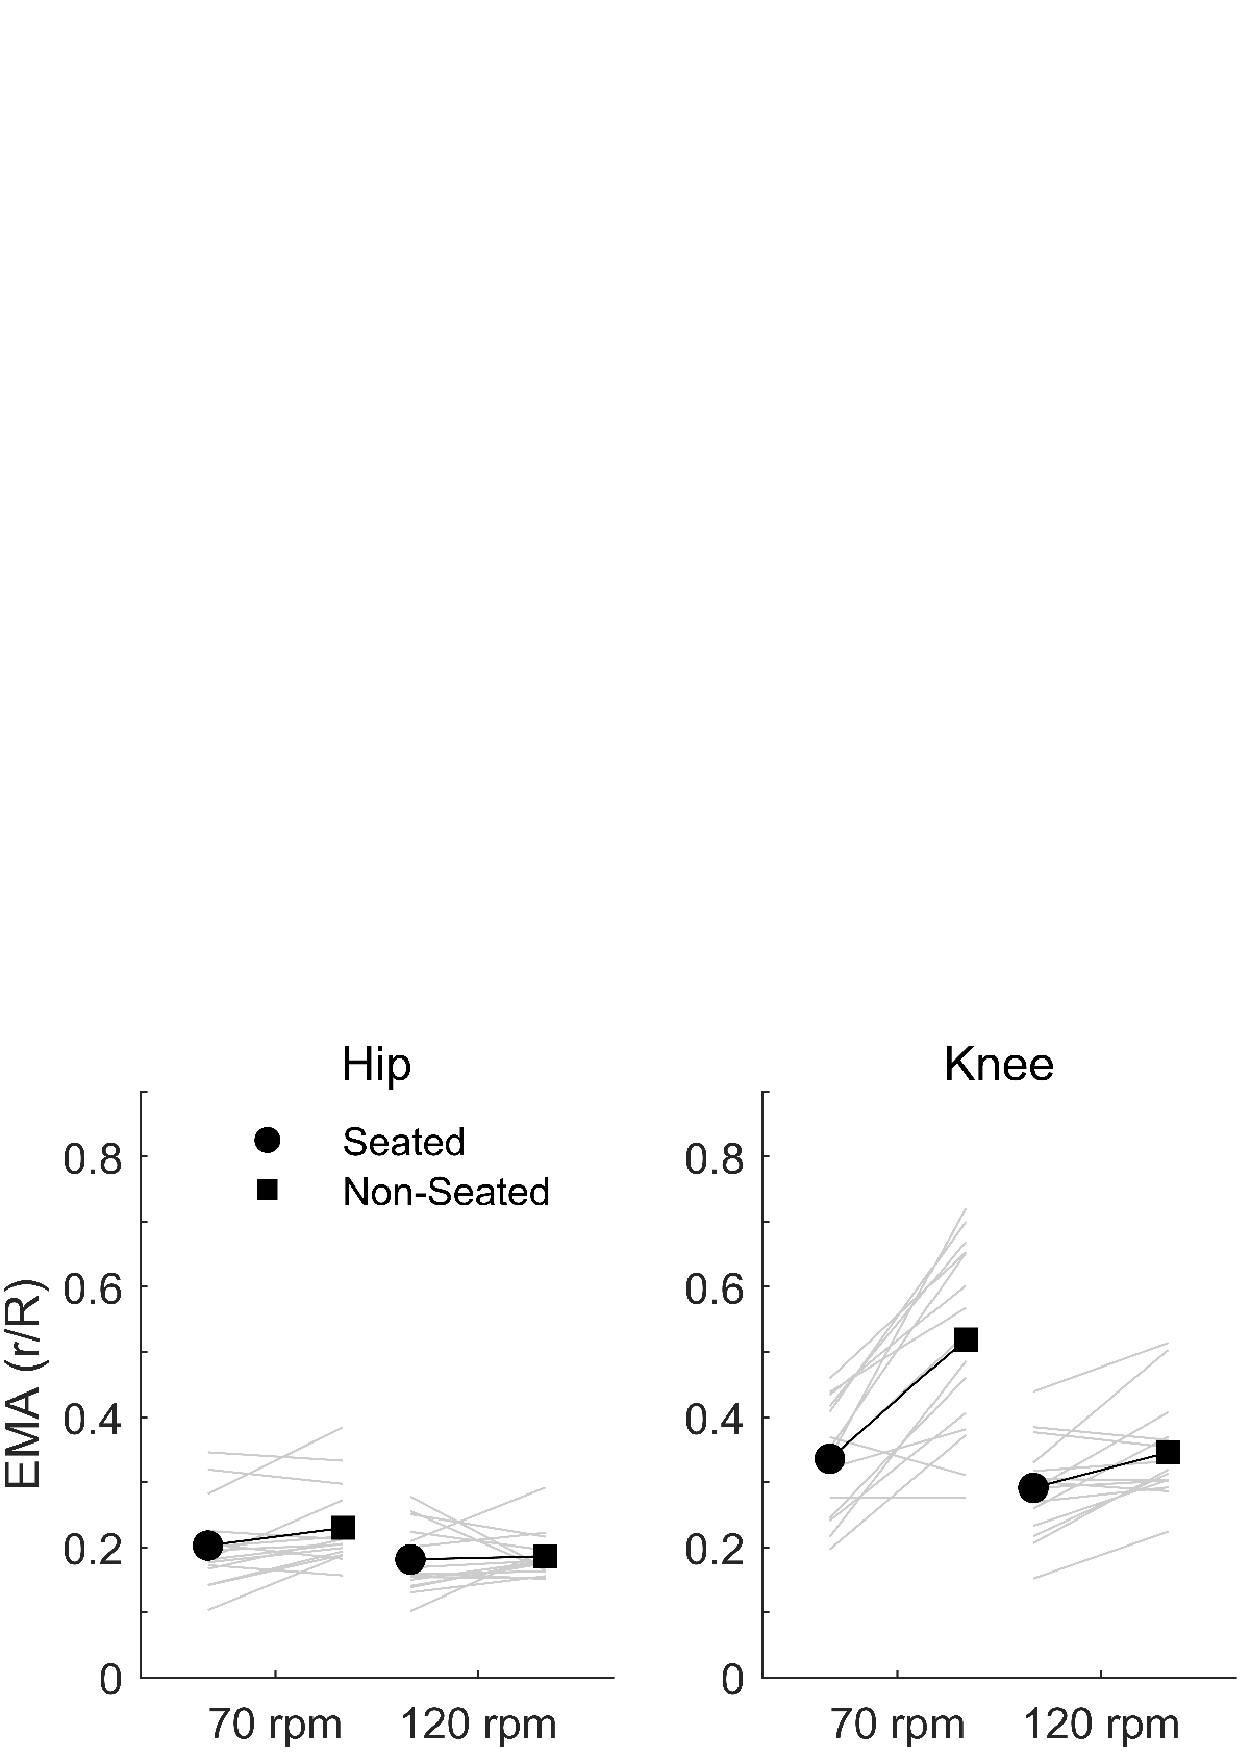
\includegraphics[width=\textwidth]{LitReview/Figure4.png}
        \caption[The effects of changing cadence and/or power output on crank torque are each unique depending on the power output and cadence you're riding at.]{\textbf{The effect of changing cadence or power output on torque requirements during cycling are each unique depending on the power and cadence you're riding at.} Top: A surface plot of torque as a function of power and cadence. Bottom left: Torque as a function of cadence. Bottom right: Torque as a function of power. The effect of changing power output on torque requirements is linear, but greater at low cadence than high cadence as can be seen by the increased slope. The effect of changing cadence on torque requirements is exponential, but increases at a greater rate as you increase power output from 50-1000 Watts. \textit{Data calculated using Equation \ref{eq:Tcranks}.}}.
            \label{fig:torque}
    \end{figure}
    \FloatBarrier

%%%%%%%%%%%%%%%%%%%%%%%%%%%%%%%%%%%%%%%%%%%%%
\section{Part III}
%%%%%%%%%%%%%%%%%%%%%%%%%%%%%%%%%%%%%%%%%%%%%
\subsection{Balance and steering}
    Maintaining balance is essential to any cycling task. Luckily, many of us gained the ability to balance a bicycle early in our childhood. Thus, the ease of performing the task later in life can mask its complexity. The principles that govern the stability of the bicycle are far from simple. Precise rider inputs must harmonise with the self-stabilising mechanisms of the bicycle \autocite{Jones1970}. To achieve balance, the bicycle and rider act as one system. The contact points between the road and the two tyres create the system's base of support (BoS). This provides a large lengthwise BoS, but a very small lateral BoS. During dynamic balance, the position and velocity of a system's CoM relative to its BoS is key \autocite{Hof2005}. If the CoM falls outside the BoS, we are able to use force to redirect the momentum of the CoM back towards the BoS. You could liken this to a gymnast moving their arms and trunk to restore balance on a beam. 
    
    Recent research has quantified the skill of balancing on a bicycle \autocite{Cain2016}. Subjects rode an instrumented bicycle on training rollers. Rollers constrain forward motion of the bicycle, but allow lateral movement and lean of the bicycle. Thus, a rider maintains balance by pedalling, steering, and leaning, similar to riding outdoors \autocite{Dressel2012}. This research compared the control strategies of experienced cyclists and non-cyclists. They graded performance on the correlation between the lateral position of CoM and the centre of pressure. At high speeds, experienced riders showed a higher correlation compared to novice riders. Meaning that experienced cyclists made small corrections to their CoM position rather than steering angle to achieve superior performance. 
    
    These researchers also measured the angle of bicycle lean in the frontal plane. This showed a negative correlation between rider lean and bicycle lean. This means that riders tend to counteract lean of the bicycle by shifting their CoM laterally or vice versa. Amplification of this motion occurs when a cyclist rides out of the saddle to climb or sprint. As the rider's produce peak force on each pedal, the bicycle steers and leans from side to side underneath the rider to shift the BoS and maintain dynamic balance of the system.
        
\subsection{Lateral bicycle dynamics}
    Lateral bicycle dynamics involve changes in the net torque acting around the longitudinal axis of the bicycle-rider system's line of support. If the equilibrium of torque is disrupted, often referred to as a toppling torque \autocite{Loram2004,Day2013}, then the system will either fall over or turn towards the fall. If the system has forward motion, then turning corners is achieved by maintaining a toppling torque on one-side of the BoS. Maintaining a straight path is achieved by continual adjustment of the toppling torque back to equilibrium. 
    
    Greater amounts of bicycle lean seem to occur when cyclists produce high pedal forces while in a non-seated posture \autocite{Duc2008} and appears to have an important role in balancing the torque around the longitudinal axis of the bicycle-rider system. Besides its apparent role during dynamic balance, little is known about how bicycle lean affects efficiency or maximal power output during cycling. 
    
    One aspect of non-seated cycling performance that should be considered is the increase in path length that is caused by the greater amplitudes of steering angle and bicycle lean. Theoretically, increasing deviations away from the straight line path between two points should increase the time it takes to complete the journey. Thus, a comparison of the effects of bicycle lean on the path length travelled during sprinting and climbing was undertaken. The results of this comparison are presented in Appendix \ref{Chap:A}.
    
    When the bicycle leans, the position of the pedals change in relation to the rider. Thus, it seems reasonable to suggest that this could change the kinematics of the rider's lower limbs. Early research using cine-film showed that the greatest angle of bicycle lean occurred when the cranks were in a vertical position \autocite{Soden1978}. This coincided with the lowest vertical position of the lower back relative to the bike frame. It was surprising that the authors of this study concluded that these motions were of little consequence to cycling performance.
    
    As the cranks are attached to the bicycle frame, the angle of lean must be the same for both. This could result in the pedal trajectory becoming elliptical rather than circular relative to the global reference frame and viewed in the sagittal plane. Very few studies have focused on the effects of bicycle lean on performance or the underlying physiological or biomechanical factors during non-seated cycling. One study tested the effect of bicycle lean on lower limb muscle activity by comparing non-seated cycling on a treadmill against cycling in a stationary ergometer which constrains bicycle lean. Their results showed that the sum of lower limb muscle activity was greater when riding the ergometer compared to using a preferred amount of lean on the treadmill \autocite{Duc2008}. Thus, bicycle lean may benefit performance by changing the conditions under which muscles must produce force and power.
    
    Bicycle lean angles were also found to increase as the slope of the ground increased \autocite{Duc2008}. The authors conclude that this is ``in order to achieve a better balance''. However, it is hard to ascertain what is meant by ``better balance'' and what aspect of slope would cause a greater demand on lateral stability if cadence and power output are kept constant. A more thorough analysis of this finding coupled with the knowledge of lateral bicycle dynamics \autocite{Kooijman2009} may help to explain these findings. When we steer and the lean the bicycle, the imaginary line between the contact point of the front and rear wheel rotates like a horizontal pendulum \autocite{Dong2014}. The projection of the rider's CoM must remain over this imaginary line of support or have a velocity in the direction of this line of support in order to maintain dynamic balance. As slope increases, the vertical projection of the bicycle's wheel base decreases. The vertical projection of the rider's CoM down to the surface of the Earth must always be in line with gravity. Therefore, the projection of the rider's CoM will move further towards the rear wheel unless the rider moves their CoM forward towards the handlebar. If the projection of the CoM moves further back in the wheel base, then an important change occurs regarding the amount of steering and lean that is required to bring the line of support underneath the CoM. As slope increases, the same lateral shift of the CoM will require greater and greater angular changes to the line of support. Hence, a greater amount of steering and subsequent lean would be required. An investigation of rider CoM position during non-seated cycling on increasing slopes would be necessary to show the relationship between slope, balance requirements, and bicycle lean angles. In such a study it would be necessary to measure the following: 1) the slope of the ground, 2) the fore-aft position of CoM within the bicycle's wheelbase, 3) the height of the rider's CoM above the ground, 4) the heading angle of the bicycle's line of support, and 5) the roll angle of the bicycle.
    
    Leaning the bicycle also causes a vertical displacement of the bicycle's CoM. It is conceivable that the magnitude and timing of bicycle lean could decrease the vertical displacement of the bicycle-rider system's CoM. Out-of-phase vertical displacement between the rider and bicycle's CoM could play an important role in sprint cycling performance. Evidence for the benefit of this decoupling motion comes from research on the modern racing position of jockeys \autocite{Pfau2009}. This research shows that adopting the modern riding technique allows jockeys to reduce the system's CoM movement in a global reference frame by moving their CoM out-of-phase with the horse's CoM. To do this the jockey performs a high amount of negative mechanical work with their legs \autocite{Pfau2009}. This dissipation of energy compensates for the gain in potential energy of the horse. The result is that the horse no longer needs to perform work to raise and lower the mass of the jockey during each stride. The adoption of this technique over the first decade of the 20$^{th}$ century led to a greater improvement of race times in one decade than that of the following century \autocite{Pfau2009}. It remains unclear whether a similar out-of-phase motion between the rider and bicycle's CoM occurs during non-seated cycling and whether it can provide any performance advantages.
    
\subsection{Stability of a bicycle on treadmills and rollers}
    As outlined by Meijaard et al. (2011) in their ``Historical Review of Thoughts on Bicycle Stability'', there are many common beliefs about the stability of bicycles that are in contrast to reality. For example, neither the ``gyro effect'' nor trail of the front wheel behind the steering axis are necessary for a bicycle to self-stabilise. Instead, their findings highlight a complex interaction of many other terms. Specifically, they concluded that the location of the front-assembly CoM relative to the system CoM and steer axis was the one variable that had the greatest effect on self-stability. There findings have particular significance for conducting experiments on treadmills and rollers. An assumption that pervades cycling research is that lateral dynamics of a bicycle are different when riding on a treadmill compared to riding outdoors. However, rigorous experimental findings \autocite{Kooijman2009} together with the principle of Galilean invariance \autocite{Dressel2012} show that at constant velocity, riding a bicycle on a treadmill is mechanically identical to riding on fixed, level ground. The original example used to illustrate that the laws of motion hold true in all inertial reference frames was that of a passenger below the deck of a ship travelling at constant velocity without rocking \autocite{Galilei1632}. In the passenger's frame of reference the ship appears to be stationary, thus they would be unable to distinguish whether the ship had a velocity or was stationary. It is obvious in this example that the passenger's frame of reference has no bearing on the laws of motion acting on the ship. Similarly, the frame of reference of a rider or an observer during treadmill cycling has no bearing on the laws of motion acting on the bicycle. 
    
    There are however subtle differences between riding on rollers compared to riding on a treadmill and fixed ground \autocite{Dressel2012}. First, the curved surface of the rollers means that the contact patch of a tyre on rollers is less than on a flat treadmill belt. Secondly, there is a \textit{``complex geometric interaction between the front wheel and the upper surface of the front roller as the bicycle steers and yaws''}, which requires further investigation to be fully understood. Finally, \textit{``the moments about a vertical axis exerted on the rear wheel by lateral forces''} differs from treadmill cycling as the rear wheel is in contact with two rollers rather than a flat belt. 
        
    Beyond the mechanics there are alterations to psychological factors and motion perception that pertain to riding on both a treadmill and rollers that may increase the difficulty of the task. First, the narrow width of the belt or rollers constrain the rider to an unusually narrow path and may induce a cognitive dissonance between the expectation or sense of moving forward and the stationary visual field. The presence and magnitude of these effects is still unknown, however it must be considered when attempting to generalise findings from studies on treadmills and rollers to riding on a fixed surface.
    
\subsection{Effect of bicycle lean on the metabolic cost of cycling}
    Literature on this topic is sparse, however it has been proposed by one group of authors that cyclists may be able to decrease the metabolic cost of cycling in a non-seated posture by self-restricting the amount of lateral bicycle lean that occurs during each crank cycle \autocite{Bouillod2018}. This theory was proposed after finding that both metabolic cost and bicycle lean velocity increased during uphill cycling in a non-seated posture versus a seated posture. The obvious flaw in this theory is the confounding effect of posture. The non-seated posture increases both metabolic energy expenditure and bicycle lean velocity. Thus, this spurious correlation provides no evidence of any relationship between bicycle lean velocity and metabolic cost. Furthermore, this investigation had a number of methodological flaws. First, metabolic measures were taken during 30-s intervals of cycling where riders immediately switched from a seated to non-seated posture. To illustrate the problem of inferring the metabolic cost during interval type training sessions, consider measuring metabolic cost on someone performing alternating 30-s bouts of cycling at 100 W and 300W in the same posture. The well-known delay between mechanical power production and oxygen uptake \autocite{Astrand2003} means that we could make erroneous conclusions about the metabolic cost of each intensity as a washout period occurs during each 30-s interval. Secondly, the RER values in this experiment were $>$1, meaning that the ratio of CO$_2$ exceeded that of O$_2$. This invalidates any conclusions about metabolic energy expenditure, as the predominant fuel source was supplied through anaerobic metabolism during all conditions \autocite{Astrand2003}. Finally, as mentioned, there was no direct comparison between a non-seated posture with and without the use of bicycle lean. Therefore, the spurious correlation between bicycle lean velocity and metabolic energy expenditure is likely due to differences between the seated and non-seated posture. To the best of our knowledge, no other evidence has been published regarding the direct effect of self-restricting bicycle lean on the mechanics or energetics of non-seated cycling.